\chapter{Аналитическая часть}
\section{Электронная цифровая подпись}

Электронная (цифровая) подпись --- ЭЦП --- позволяет подвердить авторство электронного документа. Она связана не только с автором документа, но и с самим документов (при помощи криптографических методов) и не может быть подделана при поммощи обычного копирования.

Создание ЭП с использованием криптографического алгоритма RSA и алгоритма хеширования SH1/MD5 происходит следующим образом:
\begin{enumerate}[label=\arabic*)]
	\item происходит хеширование сообщения при помощи SH1/MD5, сообщение --- файл, который неообходимо подписать;
	\item происходит шифрование с использованием закрытого ключа RSA последовательности 128/160 бит, полученных на предыдущем этапе;
	\item значение подписи --- результат шифрования.
\end{enumerate}

Проверка ЭП с использованием криптографического алгоритма RSA и алгоритма хеширования MD5 происходит следующим образом:
\begin{enumerate}[label=\arabic*)]
	\item происходит хеширование сообщения при помощи SH1/MD5, сообщение --- файл, подпись которого необходимо проверить;
	\item происходит расшифровка
	 подписи с использованием открытого ключа RSA;
	\item происходит побитовая сверка значений, полученных на предыдущих этапах, если они одинаковы, подпись считается подлинной.
\end{enumerate}

\section{Алгоритм RSA}

RSA (аббревиатура от фамилий Rivest, Shamir и Adleman) --- ассиметричный алгоритм с открытым ключом, основывающийся на вычислительной сложности задачи факторизации больших полупростых чисел. В алгоритме RSA используется 2 ключа --- открытый (публичный) и закрытый (приватный).

В ассиметричной криптографии и алгоритме RSA, в частности, открытый и закрытый ключи являются двумя частями одного целого и неразрывны друг с другом. Для шифрования информации используется открытый ключ, а для её расшифровки закрытый.

Криптосистема RSA стала первой системой, пригодной и для шифрования, и для цифровой подписи. Алгоритм используется в большом числе криптографических приложений, включая PGP, S/MIME, TLS/SSL, IPSEC/IKE и других.

RSA ключи генерируются следующим образом:
\begin{enumerate}[label=\arabic*)]
	\item выбираются два отличающихся друг от друга случайных простых числа $p$ и $q$, лежащие в установленнном диапазоне;
	\item вычисляется их произведение $n = p \cdot q$, называемое модулем;
	\item вычисляется значение функции Эйлера от числа $n$: $\phi(n) = (p - 1)\cdot (q - 1)$;
	\item выбирается целое число $e$ ($1 < e < \phi(n)$), взаимно простое со значением $\phi(n)$, оно называется открытой экспонентой;
	\item вычисляется число $d  = e^{-1} mod (\phi(n))$, оно называется закрытой экспонентой.
\end{enumerate}

Пара $(e, n)$ публикуются в качестве открытого ключа RSA, а пара $(d, n)$ --- в виде закрытого ключа.


Шифрование сообщения $m$ ($0 < m < n - 1)$ в зашифрованное сообщение $c$ производится по формуле $ c = E(m, k_1) = E(m, n, e) = m^{e} mod (n)$.

Расшифрация: $m = D(c, k_2) = D(c, n, d) = c^{d} mod (n)$

У данного принципа имеется следующие минусы:
\begin{enumerate}[label=\arabic*)]
	\item если $m = 0$, то и $c = 0$;
	\item если $m_1 = m_2$, то и $c_1 = c_2$.
\end{enumerate}

Из-за этого RSA используется для передачи ключей других шифров.

\begin{figure}[ht!]
	\centering
	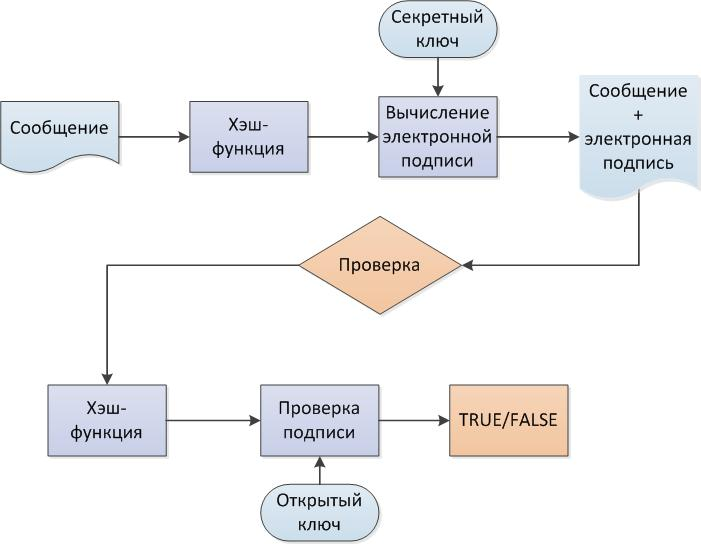
\includegraphics[width=0.8\linewidth]{img/rsa-1.jpeg}
	\caption{RSA}
	\label{img:g_function}
\end{figure}

\section{Алгоритм MD5}

MD5 (англ. \textit{Message Digest 5}) --- алгоритм хеширования, предназначенный для получения последовательнсти длиной 128 бит, используемой для последующей проверки подлинности сообщений произвольных длины.

На вход алгоритма поступает последовательность бит произвольной длины $L$, хеш которй нужно найти. 
Алгоритм MD5 состоит из 4 следующих этапов
\begin{enumerate}[label=\arabic*)]
	\item выравнивание потоков;
	\item добавление длины сообщения;
	\item инициализация буфера;
	\item вычисления в цикле.
\end{enumerate}

Выравнивание потоков представляет из себя добавление некоторого числа нулевых бит такое, чтобы новая длина последовательности $L'$ стала сравнима с 448 по модулю 512. Выравнивание происходит в любом случае, даже если длина исходного потока уже сравнима с 448

Под добавлением длины сообщения представляет из себя добавление 64 битов в последовательность: сначала младшие 4 байта, потом старшие 4 байта. После этого длина потока станет кратной 512. Вычисления будут основываться на представлении этого потока данных в виде массива слов по 512 бит.

После этого происходит инициализация буфера, состоящего из 4-х переменных размерностью 32 бита, начальные значения которых задаются шестнадцатеричными числами.
В этих переменных будут храниться результаты промежуточных вычислений.

Далее в цикле каждый блок длиной 512 бит проходит 4 этапа вычислений по 16 раундов. Для этого блок представляется в виде массива $X$ из 16 слов по 32 бита.
Все раунды однотипны и имеют вид: [abcd k s i], определяемый как $a = b + ((a +Fun(b, c,d) + X[k] + T[i]	) << s)$, где $k$ --- номер 32-битного слова из текущего блока, число $s$ задаётся отдельно для каждого раунда, $T$ --- таблица констант.

Результат вычислений хранится в переменных  $a$, $b$, $c$ и $d$.
